%%%%%%%%%%%%%%%%%%%%%%%%%%%%%%%%%%%%
%% Template file SP 2024
%% Include in directory homework.sty and headerfooter.tex
%%%%%%%%%%%%%%%%%%%%%%%%%%%%%%%%%%%%

\documentclass[12pt]{article}
\usepackage{homework}

\graphicspath{{images/}}
\geometry{letterpaper, portrait, includeheadfoot=true, hmargin=1in, vmargin=1in}

\setcounter{section}{-1}
%% Solution hiding %%
\usepackage[utf8]{inputenc}
\usepackage{lipsum}

\begin{document}
\singlespacing

\renewcommand{\familydefault}{\rmdefault}
\pagestyle{fancy}
\fancyhf{}
\setlength{\headheight}{30pt}
\renewcommand{\headrulewidth}{0.4pt}
\renewcommand{\footrulewidth}{0.4pt}
\lhead{\large Homework 2 \\ Due Feb. 20, 2024 }
\rhead{\large CS 446 \\ Spring 2024}
\rfoot{\textbf{Page \thepage}}
\lfoot{}

\section{Instructions}

Homework is due Tuesday, February 20, 2024 at 23:59pm Central Time.
Please refer to \url{https://courses.grainger.illinois.edu/cs446/sp2024/homework/hw/index.html} for course policy on homeworks and submission instructions.

\section{Soft-margin SVM: 4pts}
Referring to hard-margin case, soft-margin SVM can be simplified in such form:
\[\min_{\boldsymbol{w} \in \mathbb{R}^d,\boldsymbol{\xi} \in \mathbb{R}^n_{\geq 0}} 
\max_{\boldsymbol{\alpha} \in \mathbb{R}^n_+, \boldsymbol{\beta} \in \mathbb{R}^n_+} 
\sum_{i \in [n]} \alpha_i (1 - \xi_i - y^{(i)} \boldsymbol{w}^{\top} \boldsymbol{x}^{(i)}) 
+ \sum_{i \in [n]} -\beta_i \xi_i
+ \frac{\lambda}{2}\|\boldsymbol{w}\|_2^2
+ C \sum_{i \in [n]}\xi_i\]
with constraints:
\[y^{(i)} \boldsymbol{w}^{\top} \boldsymbol{x}^{(i)} \geq 1 - \xi_i
,\quad
\xi_i \geq 0\]
and thus we have the dual problem:
\[D(\boldsymbol{\alpha}) = 
\min_{\boldsymbol{w} \in \mathbb{R}^d,\boldsymbol{\xi} \in \mathbb{R}^n_{\geq 0}} 
\sum_{i \in [n]} \alpha_i (1 - \xi_i - y^{(i)} \boldsymbol{w}^{\top} \boldsymbol{x}^{(i)})
+ \sum_{i \in [n]} -\beta_i \xi_i
+ \frac{\lambda}{2}\|\boldsymbol{w}\|_2^2
+ C \sum_{i \in [n]}\xi_i\]
For the gradient of the problem with respect to $\boldsymbol{w}$:
\[\nabla_{\boldsymbol{w}}
\sum_{i \in [n]} \alpha_i (1 - \xi_i - y^{(i)} \boldsymbol{w}^{\top} \boldsymbol{x}^{(i)})
+ \sum_{i \in [n]} -\beta_i \xi_i
+ \frac{\lambda}{2}\|\boldsymbol{w}\|_2^2
+ C \sum_{i \in [n]}\xi_i
= 0\]
\[\Rightarrow \boldsymbol{w} = \sum_{i \in [n]} \alpha_i y^{(i)} x^{(i)}\]
For the gradient of the problem with respect to $\boldsymbol{\xi}$:
\[\nabla_{\boldsymbol{\xi}}
\sum_{i \in [n]} \alpha_i (1 - \xi_i - y^{(i)} \boldsymbol{w}^{\top} \boldsymbol{x}^{(i)})
+ \sum_{i \in [n]} -\beta_i \xi_i
+ \frac{\lambda}{2}\|\boldsymbol{w}\|_2^2
+ C \sum_{i \in [n]}\xi_i
= 0\]
\[\Rightarrow \beta_i = C - \alpha_i\quad(\beta_i\geq0)\]
Therefore, the dual form of soft-margin SVM will be:
\[\max_{\alpha_{i,j} \in [0, C]}
\sum_{i \in [n]} \alpha_i - 
\frac{1}{2}\sum_{i,j \in [n]}\alpha_i\alpha_j y^{(i)} y^{(j)} 
\boldsymbol{x}^{(i)\top} \boldsymbol{x}^{(j)}\]
\newpage

\section{SVM, RBF Kernel and Nearest Neighbor: 6pts}
\begin{enumerate}
    \item \[\hat{\boldsymbol{w}} = \sum_{i \in [n]} \hat{\alpha_i}y^{(i)}\boldsymbol{x}^{(i)}\]
    \[\Rightarrow f(\boldsymbol{x}) = \hat{\boldsymbol{w}}^{\top}\boldsymbol{x}
    = \sum_{i \in [n]} \hat{\alpha_i}y_i\boldsymbol{x}_i^{\top}\boldsymbol{x}\]
    \item \[f_\sigma(\boldsymbol{x}) = \hat{\boldsymbol{w}}^{\top}\kappa(\boldsymbol{x}_i, \boldsymbol{x}_j)
    = \sum_{i \in [n]} \hat{\alpha_i}y_i \exp \left( -\frac{\|\boldsymbol{x}_i - \boldsymbol{x}_j\|_2^2}{2\sigma^2} \right)\]
    \item \[f_\sigma(\boldsymbol{x}) = \hat{\boldsymbol{w}}^{\top}\kappa(\boldsymbol{x}_i, \boldsymbol{x}_j)
    = \sum_{i \in S} \hat{\alpha_i}y_i \exp \left( -\frac{\|\boldsymbol{x}_i - \boldsymbol{x}_j\|_2^2}{2\sigma^2} \right)\]
    \[= \sum_{i \in T} \hat{\alpha_i}y_i \exp \left( -\frac{\|\boldsymbol{x}_i - \boldsymbol{x}_j\|_2^2}{2\sigma^2} \right)
    + \sum_{i \in S\backslash T} \hat{\alpha_i}y_i \exp \left( -\frac{\|\boldsymbol{x}_i - \boldsymbol{x}_j\|_2^2}{2\sigma^2} \right)\]
    \[= \sum_{i \in T} \hat{\alpha_i}y_i \exp \left( -\frac{\rho^2}{2\sigma^2} \right)
    + \sum_{i \in S\backslash T} \hat{\alpha_i}y_i \exp \left( -\frac{c}{2\sigma^2} \right)\] 
    \[\Longrightarrow \frac{f_\sigma(\boldsymbol{x})}{\exp\left(-\rho^2/2\sigma^2\right)}
    = \sum_{i \in T} \hat{\alpha_i}y_i + \sum_{i \in S\backslash T} \hat{\alpha_i}y_i \exp \left(\frac{\rho^2 - \|\boldsymbol{x}_i - \boldsymbol{x}\|_2^2}{2\sigma^2} \right)\]
    Since:
    \[\forall i \in S\backslash T,\: \rho^2 < \|\boldsymbol{x}_i - \boldsymbol{x}_j\|_2^2\]
    we have the limit:
    \[\lim_{\sigma\rightarrow0}\frac{\rho^2 - \|\boldsymbol{x}_i - \boldsymbol{x}\|_2^2}{2\sigma^2}\rightarrow-\infty\]
    hence:
    \[\lim_{\sigma\rightarrow0} \frac{f_\sigma(\boldsymbol{x})}{\exp\left(-\rho^2/2\sigma^2\right)}
    = \lim_{\sigma\rightarrow0}
    \sum_{i \in T} \hat{\alpha_i}y_i + \sum_{i \in S\backslash T} \hat{\alpha_i}y_i \exp \left(\frac{\rho^2 - \|\boldsymbol{x}_i - \boldsymbol{x}\|_2^2}{2\sigma^2} \right)\] 
    \[= \sum_{i \in T} \hat{\alpha_i}y_i + 0 = \sum_{i \in T} \hat{\alpha_i}y_i\]
\end{enumerate}
\newpage

\section{Decision Tree and Adaboost: 12 pts}
\begin{enumerate}
    \item \[I(\mathcal{D}) = - \sum_{y\in{-1,1}}p(y|\mathcal{D})\log_2 p(y|\mathcal{D})\]
    \[= -p(1|\mathcal{D})\log_2p(1|\mathcal{D}) -p(-1|\mathcal{D})\log_2p(-1|\mathcal{D})\]
    \[= -\frac{1}{2}\log_2\frac{1}{2} - \frac{1}{2}\log_2\frac{1}{2} = 1\]
    \item rule: $f_1: x_1\geq4.5$\\
    information gain with 3 green 1 blue v.s. 2 blue:
    \[IG(\mathcal{D},f_1) = I(\mathcal{D}) - \sum_{j=1}^{2}\frac{|\mathcal{D}_j|}{|\mathcal{D}|}I(\mathcal{D}_j)\]
    \[= 1 - \frac{4}{6}I(\mathcal{D}_1) - \frac{2}{6}I(\mathcal{D}_2)
    = 1 - \frac{2}{3}(-\frac{3}{4}\log_2\frac{3}{4} - \frac{1}{4}\log_2\frac{1}{4}) - \frac{1}{3}(-\log_2 1)\]
    \[= \frac{1}{2}\log_2 3 - \frac{1}{3}\]
    \item rule (for the left node holding $\mathcal{D}_1$):
    $f_2: x_2<1.5$\\
    In the left node, information gain with 3 green v.s. 1 blue:
    \[IG(\mathcal{D}_1,f_2) = I(\mathcal{D}_1) - I(\mathcal{D}_1|f_2)\] 
    Since all samples are in perfect split in $\mathcal{D}_1$ with $f_2$, we have:
    $I(\mathcal{D}_1|f_2) = 0$. Thus,
    \[IG(\mathcal{D}_1, f_2) = I(\mathcal{D}_1) = -\frac{3}{4}\log_2\frac{3}{4} - \frac{1}{4}\log_2\frac{1}{4} = 2 - \frac{3}{4}\log_2 3\]
    For the right node holding $\mathcal{D}_2$, since the first split has already been perfect for all samples, there's no need for the second split and thus the information gain of the second split equals to 0.
    \item For iteration $t = 1$, $f_1:x_j\geq4.5$:
    \[\gamma_1 = [\frac{1}{6}, \frac{1}{6},\frac{1}{6},\frac{1}{6},\frac{1}{6},\frac{1}{6},\frac{1}{6}]^{\top}\]
    \[\epsilon_1 = \frac{\sum_{i:y^{(i)}\neq f_1(\boldsymbol{x}^{(i)})}\gamma_i^1}{\sum_i\gamma_i^1} = \frac{1}{6}\]
    \[z_1 = \sum_{i=1}^6\gamma_1^{(i)}y^{(i)}f_1(\boldsymbol{x}^{(i)}) = \frac{5}{6} - \frac{1}{6} = \frac{2}{3}\]
    \[\alpha_1 = \frac{1}{2}\ln\frac{1+z_1}{1-z_1} = \frac{1}{2}\ln5\]
    \[\gamma_2^{(i)} = \frac{\gamma_1^{(i)}\exp(-\alpha_1y^{(i)}f_t(\boldsymbol{x}^{(i)}))}{Z_t}\]
    with $\gamma_1^{(i)}\exp(-\alpha_1y^{(i)}f_t(\boldsymbol{x}^{(i)})) = 5^{-\frac{1}{2}}$ for $i = 1, 3, 4, 5, 6$ and $5^{\frac{1}{2}}$ for $i = 2$, while\:$5^{\frac{1}{2}} = 5\cdot5^{-\frac{1}{2}}$. Thus,
    \[\gamma_2 = [\frac{1}{10}, \frac{1}{2}, \frac{1}{10}, \frac{1}{10}, \frac{1}{10}, \frac{1}{10}]^{\top}\]
    For iteration $t=2$, $f_2:x_j<1.5$:
    \[\epsilon_2 = \frac{\sum_{i:y^{(i)}\neq f_2(\boldsymbol{x}^{(i)})}\gamma_i^2}{\sum_i\gamma_i^2} = \frac{2\cdot\frac{1}{10}}{1} = \frac{1}{5}\]
    \[z_2 = \sum_{i=1}^6\gamma_2^{(i)}y^{(i)}f_2(\boldsymbol{x}^{(i)}) = \frac{1}{2} + 3\cdot\frac{1}{10} - 2\cdot\frac{1}{10} = \frac{3}{5}\]
    \[\alpha_2 = \frac{1}{2}\ln\frac{1+z_2}{1-z_2} = \frac{1}{2}\ln4\]
    \item Final classifier:
    \[f(\boldsymbol{x}) = \text{sign}(\alpha_1f_1(\boldsymbol{x}) + \alpha_2f_2(\boldsymbol{x}))\]
    \[=\text{sign}(\ln5\cdot\text{sign}(x_1 - 4.5) + \ln4\cdot\text{sign}(1.5 - x_2))\]
    Outcomes:
    \[f(\boldsymbol{x}^{(1)}) = \text{sign}(-\ln5 - \ln4) = -1\]
    \[f(\boldsymbol{x}^{(2)}) = \text{sign}(-\ln5 + \ln4) = -1\]
    \[f(\boldsymbol{x}^{(3)}) = \text{sign}(-\ln5 - \ln4) = -1\]
    \[f(\boldsymbol{x}^{(4)}) = \text{sign}(-\ln5 - \ln4) = -1\]
    \[f(\boldsymbol{x}^{(5)}) = \text{sign}(\ln5 - \ln4) = 1\]
    \[f(\boldsymbol{x}^{(6)}) = \text{sign}(\ln5 - \ln4) = 1\]
    Except for $\boldsymbol{x}^{(2)}$, classification of all samples are correct.
\end{enumerate}
\newpage

\section{Learning Theory: 14pts}
\begin{enumerate}
    \item As $R(h) \in [0, 1]$:
    \[\Pr(|R(h) - \hat{R}_S(h)|\geq0.05)\leq2\exp\left(-2n\cdot0.05^2\right)\]
    For $\Pr(|R(h) - \hat{R}_S(h)|\leq0.05)\geq0.95$, we need:
    \[2\exp\left(-2n\cdot0.05^2\right)\leq0.05\] 
    \[\Rightarrow n\geq-\frac{\ln0.025}{0.005} = 737.8 \quad\Rightarrow n\geq738\]
    \item
\begin{enumerate}
    \item[(a)] \[VC(\mathcal{F}_\text{affine}) = 2\]
    If there are 2 points, either they share the same class or not. If they are in the same class, 
    any line that intersect the axis not between the two points will work. If they are not different
    classes, any line that intersect the axis not between the two points will work.\\
    If there are 3 points, if the middle point is in a different class than the two others, no classifier
    will work. If the line intersect among the points, the middle point will always be classified in
    the same class with another point, which is wrong and remains so if the line is not intersecting
    among the points.
    \item[(b)] \[VC(\mathcal{F}_\text{affine}^k) = k+1\]
    With dataset:
    \[\textbf{X} = \begin{bmatrix}
        \boldsymbol{x}^{(1)\top} && 1\\
        \boldsymbol{x}^{(2)\top} && 1\\
        \vdots && \vdots\\
        \boldsymbol{x}^{(n)\top} && 1
    \end{bmatrix}\]
    parameters $\boldsymbol{w}\in\mathbb{R}^{n+1}$ and expected outputs $\textbf{Y}\in\{0, 1\}^n$,
    $\boldsymbol{w}$ is supposed to map \textbf{X} to arbitrary $\textbf{y}\in\mathbb{R}^n$,
    which leads to arbitrary \textbf{Y}. This means that column vectors of \textbf{X} are forming a
    basis of an $n$ dimensional space. To satisfy this condition, we can tell that the maximum value of
    $n$ would be $k+1$ since the number of columns of \textbf{X} is $k+1$, which means that the rank of
    \textbf{X} is at most $k+1$, and thus it can span to an at most $k+1$ dimensional space.
    \item[(c)] \[VC(\mathcal{F}_\text{cos}) \rightarrow \infty\]
    For $\cos(cx)$, we have zeros at 
    $cx = (n + \dfrac{1}{2})\pi,\:n\in\mathbb{Z}$, which we call critical points, and absolute maximums at $cx = n\pi,\:n\in\mathbb{Z}$. The classifier would divide $\textbf{X}$ into two parts corresponding to 2 classes:\[\left[\left(-\dfrac{1}{2} + 2n\right)\frac{\pi}{c},\, \left(\dfrac{1}{2} + 2n\right)\frac{\pi}{c}\right]\] and \[\left[\left(\dfrac{1}{2} + 2n\right)\frac{\pi}{c},\, \left(\dfrac{3}{2} + 2n\right)\frac{\pi}{c}\right]\]
    Note that for the points belong to the same class, there are supposed to be an even number of critical points between them, and vice versa. As $c$ grows to infinity, the two sets of intervals which are alternating will continue shrinking, and eventually tend to form a function that is neither continuous nor differentiable anywhere, which can offer either odd number or even number of critical points between arbitrary number of pairs of points that distant variously from each other simultaneously. It's worth noting that as $c$ goes to infinity, two pairs of points that share the same distance will surely share the same relation in classes. For example, for points pair \{1, 2\} and \{3, 4\}, if 1 and 2 are labeled as 1, while 3 and 4 are labeled as -1, at the same time, there are infinity points with sufficiently complicated class distribution such that drive $c$ to infinity, the four points can't be shattered. Hence, for all the datasets in which no pair of points shares the same distance in between, the largest cardinality of them as being shattered will be infinity. For example, $\textbf{X}: \{(2^n-1)\pi\:|\:n\in\mathbb{Z}_+\}$.
\end{enumerate}
\end{enumerate}
\newpage

\section{Coding: SVM, 4pts}
% Include your plot for Q5.3.
\begin{figure}[!htb]
    \begin{minipage}{0.48\textwidth}
        \centering
        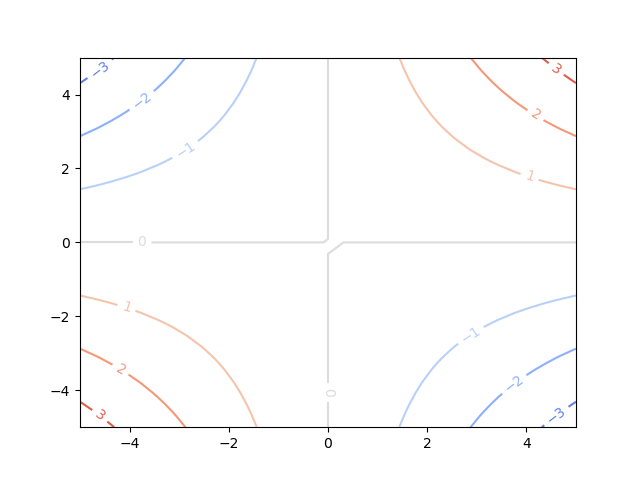
\includegraphics[width=\linewidth]{Figure_1.png}
        \caption{Polynomial kernel with degree 2}
    \end{minipage}\hfill
    \begin{minipage}{0.48\textwidth}
        \centering
        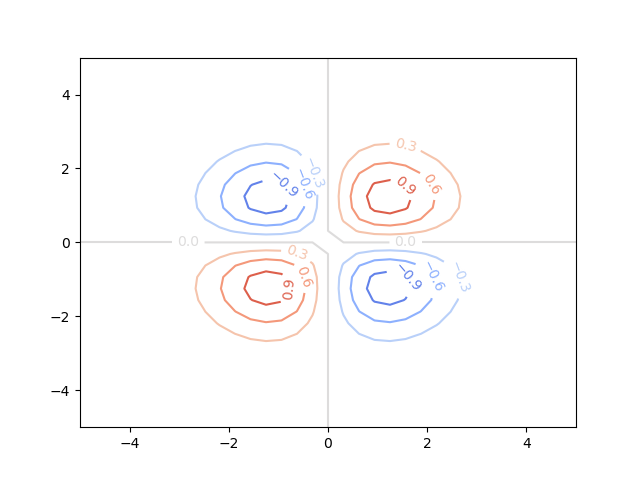
\includegraphics[width=\linewidth]{Figure_2.png}
        \caption{RBF kernel with $\sigma=1$}
    \end{minipage}\hfill
    \begin{minipage}{0.48\textwidth}
        \centering
        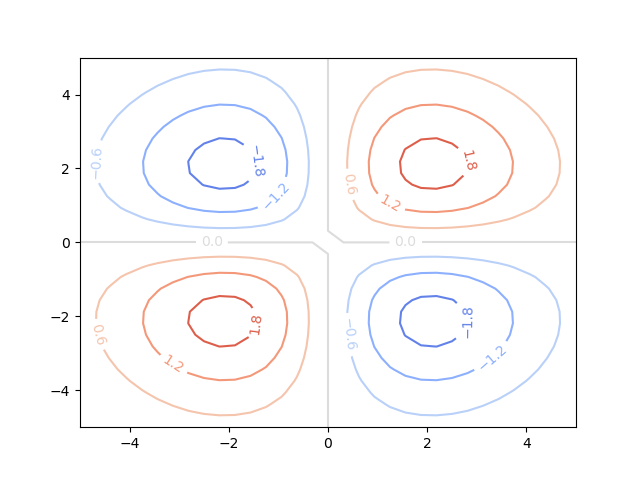
\includegraphics[width=\linewidth]{Figure_3.png}
        \caption{RBF kernel with $\sigma=2$}
    \end{minipage}\hfill
    \begin{minipage}{0.48\textwidth}
        \centering
        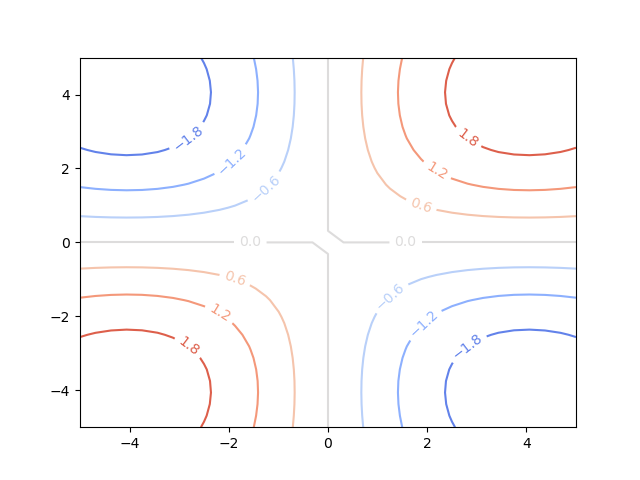
\includegraphics[width=\linewidth]{Figure_4.png}
        \caption{RBF kernel with $\sigma=4$}
    \end{minipage}
\end{figure}
\end{document}